\chapter[Арифметика с плавающей точкой. Начало]{Семинар 08. Математический сопроцессор. Арифметика с плавающей точкой}

Целью семинара является изучение подходов к реализации арифметики с плаваюющей точкой за счет применения математического сопроцессора.


На занятии предполагается рассмотреть следующие темы:
\begin{enumerate}
    \item Представление чисел с плавающей точкой.
    \item Организация математического сопроцессора в архитектуре RISC-V.
    \item Псевдоинструкции.
    \item Управление вычислениями в арифметическом сопроцессоре.
    \item Примеры вычислений с плавающей точкой.
\end{enumerate}

\section{Представление чисел с плавающей точкой}

\debate[Примечание]{Следует отметить, что формат чисел с плавающей точкой уже был рассказан на лекции. Поэтому данный материал можно было бы вообще не упоминать. Поэтому я его как бы и не упоминаю. Но можно задать вопрос о том помнят ли студенты, как представляются числа с плавающей точкой в стандарте IEEE-754.Естественно, что больше половины ничего не знают, так как игнорируют лекции. В этой ситуации я планирую просто открыть лекцию и быстро пройтись по ее содержанию одновременно с демонстрацией различных вариантов чисел (включая и крайние) на эмуляторе.}

То есть, как и Г. Курячий, обратиться к RARS и открыть окно эмулятора сопроцессора с плавающей точкой через меню (Tools->Floating Point Representaion). И в этом диалоговом окне имеется визуализация числа с плавающей точной. Можно рассмотреть, что из себя различные значения числа с плавающей точкой представляют. И как они отражаются на двоичное представление. Следует при этом учесть, что это диалоговое окно используется для отображение 32-х разрядных чисел с плавающей точкой. Поэтому, в соответствии с размерностью, ненормализованное представление начинается где-то после $10^{-38}$.

Следует подчеркнуть, что манипулировать можно не только десятичным числом, но и двоичным, выставляя знак, мантиссу и порядок. Таким образом можно показать все варианты (они отображаются в десятичном окне), включая прямое задание ненормализованных чисел, неопределенные значения, плюс/минус бесконечность.

Помимо этого во время выполнения программы данный девайс можно связать с программой и в отладочном режиме просматривать содержимое регистров с плавающей точкой (32-х разрядных значений) в десятичной системе счисления~(рисунок~\ref{fp-representation}).

\begin{figure}[htbp]
    \centering
    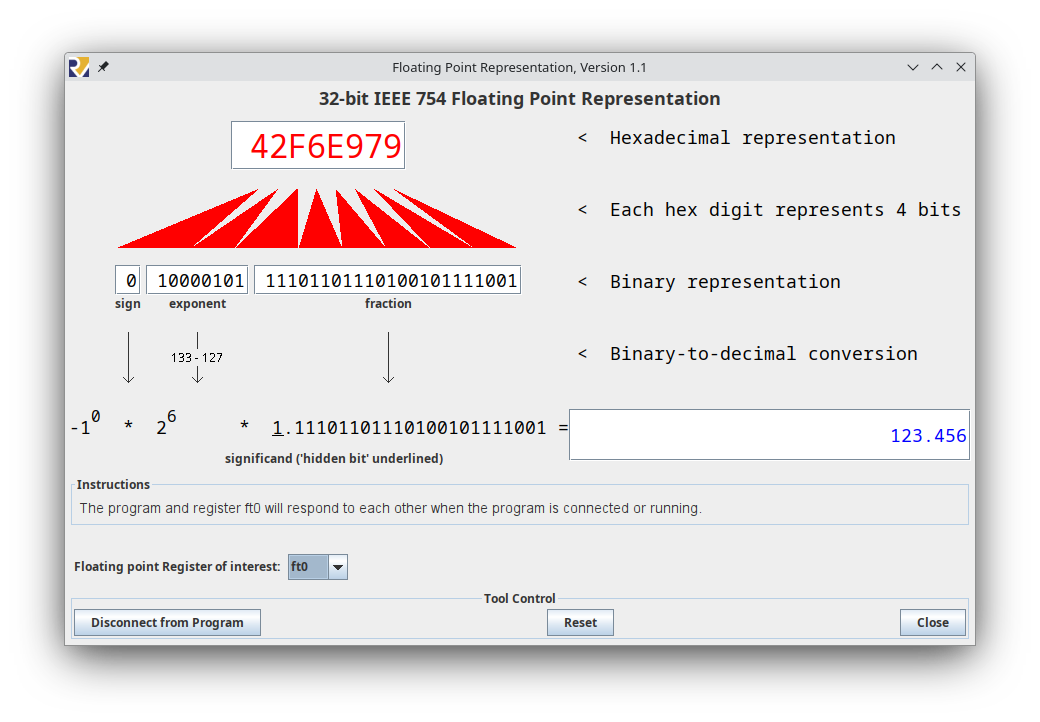
\includegraphics[width=1.0\textwidth]{img/fp-representation.png}
    \caption{Диалоговое окно для просмотра 32-х разрядных чисел с плавающей точкой}
    \label{fp-representation}
\end{figure}

\debate[Примечание]{Курячий показал только манипуляции в десятичном окне. У нас есть время показать больше. Помимо этого можно даже провести небольшое тестирование по этому поводу. Например, дать задание показать, каким образом в двоичном виде будут представлены Пи, Е, и другие числа. Включая не входящие в диапазон 32-х разрядного числа. Можно также поступить наоборот (из двоичной в десятичную), но не знаю, зачем это нужно. Хотя, я им рассказывал, что в LUA использовались ненормализованные числа для представления целочисленной арифметики (52 разряда мантиссы и знак 64-разрядного числа). Можно задать вопрос: какой диапазон целочисленной арифметики может быть представлен в 32-х разрядном числе с плавающей точкой за счет мантиссы и знака.}

\section{Организация математического сопроцессора в архитектуре RISC-V}

Можно остановится на определении сопроцессора (как и у Курячего) как дополнительного устройства, предназначенного для реализации дополнительной функциональности. Сказать, что оно может быть реализовано для различных целей и быть выполнено как на том же кристалле, что и универсальный процессор, или разработано в виде отдельного кристалла (я рассказывал об отдельном Intel 8087), или же быть отдельным устройством (например, видеокарта).

\debate[Можно немного поговорить]{Возможный вопрос: почему не использовать программное решение для арифметики с плавающей точкой на основе целочисленных регистров и моделирования на них любых форматов? Ответ: слишком медленно, а стандартные форматы с плавающей точкой обеспечивают переносимость между различными архитектурами.}

\subsection{Варианты реализации математического сопроцессора}

После этого можно перейти к особенностям математического сопроцессора в архитектуре RISC-V. Сказать, что сущeствуют различные стандарты расширения:
\begin{itemize}
    \item \textbf{F (float)} --  поддерживает числа с плавающей точкой одинарной точности (32 разряда);
    \item \textbf{D (double)} -- поддерживает числа с плавающей точкой двойной точности (64 разряда);
    \item \textbf{Q (quadruple)} -- поддерживает числа с плавающей точкой четверной точности (128 разрядов);
    \item \textbf{ZfH (half)} -- поддерживает числа с плавающей точкой половинной точности (16 разрядов).
\end{itemize}
Отметить, что RARS поддерживает стандарты \textbf{F} и \textbf{D}.

\subsection{Регистры математического сопроцессора}

Здесь содержание практически стандартно. Архитектура RISC-V предусматривает наличие тридцати двух регистров для чисел с плавающей точкой <<f0–f31>>. В математическом сопроцессоре это свои регистры, которые не связаны с регистрами процессора. Разрядность этих регистров определяется поддерживаемым стандартом расширения. В RARS это 64 разряда (double). При использовании чисел меньшей разрядности (в RARS 32 разряда) старшие части таких регистров заполняются значением \textbf{NaN} старшего числа. Тогда при попытке прочесть 64-разрядное число прочтется \textbf{NaN}.

\debate[Примечание]{Имеет смысл специально проверить при выполнении примеров.}

В соответствие с соглашением о вызове подпрограмм (\url{https://github.com/riscv-non-isa/riscv-elf-psabi-doc/blob/master/riscv-cc.adoc}), у этих регистров разное назначение (рисунок~\ref{fp-registers}).

\begin{figure}[htbp]
    \centering
    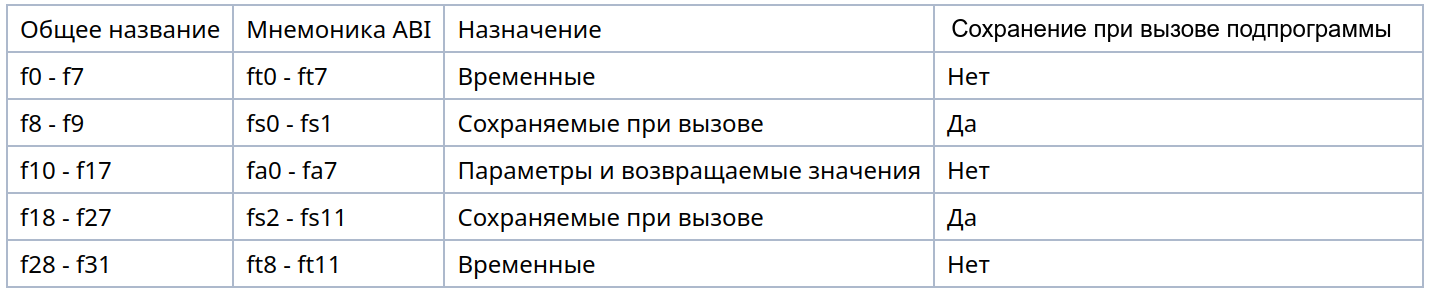
\includegraphics[width=1.0\textwidth]{img/fp-registers.png}
    \caption{Соглашения по использованию регистров с плавающей точкой}
    \label{fp-registers}
\end{figure}

Можно отметить, что в целом за счет отсутствия специализации, количество используемых регистров больше. Но при этом также заметить, что это расширение процессора. То есть, дополнительное устройство внутри кристалла. Следовательно, оно создается в случае более мощных процессоров и не присутствует в микроконтроллерах, которым оно не нужно из-за специфики их применения.

\subsection{Система команд математического сопроцессора}

\debate[Примечание]{Я разбил команды по группам на будущее. Возможно, что не совсем корректно и без перевода. Но думаю, что при формировании более сложной методы это можно будет повторно использовать.}

\subsubsection{Команды обработки данных арифметического сопроцессора}
Команды обработки данных арифметического сопроцессора представлены в таблице~\ref{table-fp-processor-calc}

\begin{table}[h]
    \caption{Команды обработки данных арифметического сопроцессора}
    \centering
    \begin{tabularx}{\textwidth}{|l|X|}
        \hline
        \textbf{Команда} & \textbf{Описание} \\
        %\hline  \multicolumn{3}{|c|}{\textbf{\textit{Арифметические}}} \\
        \hline \verb|fadd.d f1, f2, f3, dyn| & Floating ADD (64 bit): assigns f1 to f2 + f3 \\
        \hline \verb|fadd.s f1, f2, f3, dyn| & Floating ADD: assigns f1 to f2 + f3 \\
        \hline \verb|fdiv.d f1, f2, f3, dyn| & Floating DIVide (64 bit): assigns f1 to f2 / f3 \\
        \hline \verb|fdiv.s f1, f2, f3, dyn| & Floating DIVide: assigns f1 to f2 / f3 \\
        \hline \verb|fmul.d f1, f2, f3, dyn| & Floating MULtiply (64 bit): assigns f1 to f2 * f3 \\
        \hline \verb|fmul.s f1, f2, f3, dyn| & Floating MULtiply: assigns f1 to f2 * f3 \\
        \hline \verb|fsgnj.d f1, f2, f3| & Floating point sign injection (64 bit): replace the sign bit of f2 with the sign bit of f3 and assign it to f1 \\
        \hline \verb|fsgnj.s f1, f2, f3| & Floating point sign injection: replace the sign bit of f2 with the sign bit of f3 and assign it to f1 \\
        \hline \verb|fsgnjn.d f1, f2, f3| & Floating point sign injection (inverted 64 bit):  replace the sign bit of f2 with the opposite of sign bit of f3 and assign it to f1 \\
        \hline \verb|fsgnjn.s f1, f2, f3| & Floating point sign injection (inverted):  replace the sign bit of f2 with the opposite of sign bit of f3 and assign it to f1 \\
        \hline \verb|fsgnjx.d f1, f2, f3| & Floating point sign injection (xor 64 bit):  xor the sign bit of f2 with the sign bit of f3 and assign it to f1 \\
        \hline \verb|fsgnjx.s f1, f2, f3| & Floating point sign injection (xor):  xor the sign bit of f2 with the sign bit of f3 and assign it to f1 \\
        \hline \verb|fsub.d f1, f2, f3, dyn| & Floating SUBtract (64 bit): assigns f1 to f2 - f3 \\
        \hline \verb|fsub.s f1, f2, f3, dyn| & Floating SUBtract: assigns f1 to f2 - f3 \\
        \hline
    \end{tabularx}
    \label{table-fp-processor-calc}
\end{table}

\subsubsection{Команды пересылки данных арифметического сопроцессора}
Команды пересылки данных арифметического сопроцессора представлены в таблице~\ref{table-fp-processor-move}

\begin{table}[h]
    \caption{Команды пересылки данных арифметического сопроцессора}
    \centering
    \begin{tabularx}{\textwidth}{|l|X|}
        \hline
        \textbf{Команда} & \textbf{Описание} \\
        %\hline  \multicolumn{3}{|c|}{\textbf{\textit{Арифметические}}} \\
        \hline \verb|fld f1, -100(t1)| & Load a double from memory \\
        \hline \verb|flw f1, -100(t1)| & Load a float from memory \\
        \hline \verb|fmv.s.x f1, t1| & Move float: move bits representing a float from an integer register \\
        \hline \verb|fmv.x.s t1, f1| & Move float: move bits representing a float to an integer register \\
        \hline \verb|fsd f1, -100(t1)| & Store a double to memory \\
        \hline \verb|fsw f1, -100(t1)| & Store a float to memory \\
        \hline
    \end{tabularx}
    \label{table-fp-processor-move}
\end{table}

\subsubsection{Команды конвертации данных арифметического сопроцессора}
Команды конвертации данных арифметического сопроцессора представлены в таблице~\ref{table-fp-processor-convert}

\begin{table}[h]
    \caption{Команды конвертации данных арифметического сопроцессора}
    \centering
    \begin{tabularx}{\textwidth}{|l|X|}
        \hline
        \textbf{Команда} & \textbf{Описание} \\
        %\hline  \multicolumn{3}{|c|}{\textbf{\textit{Арифметические}}} \\
        \hline \verb|fcvt.d.s f1, f2, dyn| & Convert a float to a double: Assigned the value of f2 to f1 \\
        \hline \verb|fcvt.d.w f1, t1, dyn| & Convert double from integer: Assigns the value of t1 to f1 \\
        \hline \verb|fcvt.d.wu f1, t1, dyn| & Convert double from unsigned integer: Assigns the value of t1 to f1 \\
        \hline \verb|fcvt.s.d f1, f2, dyn| & Convert a double to a float: Assigned the value of f2 to f1 \\
        \hline \verb|fcvt.s.w f1, t1, dyn| & Convert float from integer: Assigns the value of t1 to f1 \\
        \hline \verb|fcvt.s.wu f1, t1, dyn| & Convert float from unsigned integer: Assigns the value of t1 to f1 \\
        \hline \verb|fcvt.w.d t1, f1, dyn| & Convert integer from double: Assigns the value of f1 (rounded) to t1 \\
        \hline \verb|fcvt.w.s t1, f1, dyn| & Convert integer from float: Assigns the value of f1 (rounded) to t1 \\
        \hline \verb|fcvt.wu.d t1, f1, dyn| & Convert unsinged integer from double: Assigns the value of f1 (rounded) to t1 \\
        \hline \verb|fcvt.wu.s t1, f1, dyn| & Convert unsinged integer from float: Assigns the value of f1 (rounded) to t1 \\
        \hline
    \end{tabularx}
    \label{table-fp-processor-convert}
\end{table}


Форматы команд математического сопроцессора совпадают с форматами \textbf{S} (запись в память, fs*), \textbf{I} (чтение из памяти, fl*) и \textbf{R} (вычисления).

Для хранения и передачи данных можно использовать слова, двойные слова, так как на уровне системы команд используется операционная однозначность (однозначность выполнения операций рассматривалась на лекциях). Поэтому мнемоника комнд пересылки использует обозначения <<word>> / <<double word>>: flw, fsw, fld, fsd, (а также *q и *h, если они реализованы в соответствующих стандартах расширений архитектуры).

Точность арифметических команд сопроцессора указывается суффиксом инструкции (s, d, q, h) который в ассемблере добавляется к коду операций, отделяясь от него точкой: \verb|fCMD.P|, где \verb|CMD| — мнемоника инструкции,
\verb|P| — точность.

Примеры команд \verb|CMD: add, sub, mul, div, sqrt, min, max|

\subsubsection{Вычисление полусуммы двух чисел}

Пример от Г.Курячего, демонстрирующий основные команды, пояснения есть в видео.

\begin{verbatim}
        .data
    a:      .float  123.456
    b:      .float  654.321
    _2:     .float  2
        .text
        flw     ft0 a t0
        flw     ft1 b t0
        flw     ft2 _2 t0
        fadd.s  ft3 ft2 ft1
        fdiv.s  fa0 ft3 ft2
        li      a7 2
        ecall
\end{verbatim}
При этом какие регистры и как используются определяется кодом операции. Информация об этих командах также имеется в системе помощи RARS. Переключение на сопроцессор осуществляет устройство управления по коду операции команды. Оно также определяе использование регистров с плавающей точкой совместно с целочисленными регистрами.

Пример раскрытия  команды \verb|flw| (рисунок~\ref{flw-example}). Представлен также в видео.

\begin{figure}[htbp]
    \centering
    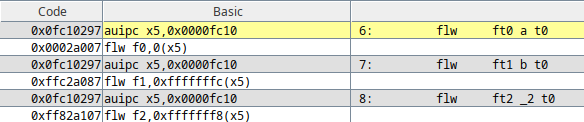
\includegraphics[width=1.0\textwidth]{img/flw-example.png}
    \caption{Раскрытие команды flw при ассемблировании}
    \label{flw-example}
\end{figure}
Также с данной программой можно пройтись пошагово. Тогда можно увидеть как меняются различные регистры. Обратить внимание на t0, используемый в данном случае для формирования базы адреса в памяти, чтобы обеспечить доступ для загрузки числа. А также отметить использование уже рассмотренной команды \verb|auipc| для формирования позиционно независимого кода. При этом можно обратить внимание, что 32-разрядные слова фиксируются в регистрах с плавающей точкой без указания старшей части, которая должна быть \textbf{NaN}.

\subsubsection{Команды арифметического сопроцессора, осуществляющие обработку сложных выражений}

Наряду с традиционными форматами команд в арифметический процессор добавлен новый тип команд \textbf{R4} (рисунок~\ref{fp-r4-type}), поддерживающих четыре операнда.

\begin{figure}[htbp]
    \centering
    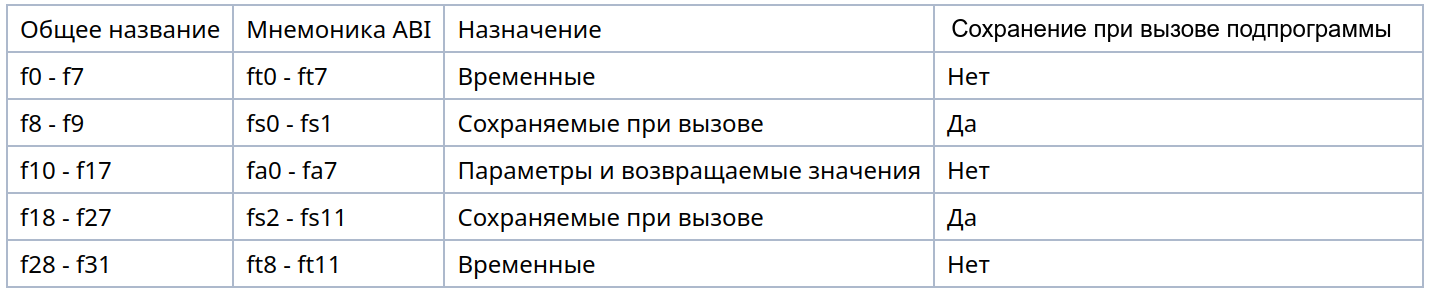
\includegraphics[width=1.0\textwidth]{img/fp-registers.png}
    \caption{Формат \textbf{R4}, используемый для поддержки составных операций}
    \label{fp-r4-type}
\end{figure}
Данные команды выполняют не элементарные действия а вычисления по более сложным выражениям с чередованием операций умножения, сложения, вычитания, смены знака. Эти команды представлены в таблице~\ref{table-fp-processor-complex}

\begin{table}[h]
    \caption{Команды арифметического сопроцессора, осуществляющие обработку сложных выражений}
    \centering
    \begin{tabularx}{\textwidth}{|l|X|}
        \hline
        \textbf{Команда} & \textbf{Описание} \\
        %\hline  \multicolumn{3}{|c|}{\textbf{\textit{Арифметические}}} \\
        \hline \verb|fmadd.d f1, f2, f3, f4, dyn| & Fused Multiply Add (64 bit): Assigns f2*f3+f4 to f1 \\
        \hline \verb|fmadd.s f1, f2, f3, f4, dyn| & Fused Multiply Add: Assigns f2*f3+f4 to f1 \\
        \hline \verb|fmsub.d f1, f2, f3, f4, dyn| & Fused Multiply Subatract: Assigns f2*f3-f4 to f1 \\
        \hline \verb|fmsub.s f1, f2, f3, f4, dyn| & Fused Multiply Subatract: Assigns f2*f3-f4 to f1 \\
        \hline \verb|fnmadd.d f1, f2, f3, f4, dyn| & Fused Negate Multiply Add (64 bit): Assigns -(f2*f3+f4) to f1 \\
        \hline \verb|fnmadd.s f1, f2, f3, f4, dyn| & Fused Negate Multiply Add: Assigns -(f2*f3+f4) to f1 \\
        \hline \verb|fnmsub.d f1, f2, f3, f4, dyn| & Fused Negated Multiply Subatract: Assigns -(f2*f3-f4) to f1 \\
        \hline \verb|fnmsub.s f1, f2, f3, f4, dyn| & Fused Negated Multiply Subatract: Assigns -(f2*f3-f4) to f1 \\
        \hline \verb|fmax.d f1, f2, f3| & Floating MAXimum (64 bit): assigns f1 to the larger of f1 and f3 \\
        \hline \verb|fmax.s f1, f2, f3| & Floating MAXimum: assigns f1 to the larger of f1 and f3 \\
        \hline \verb|fmin.d f1, f2, f3| & Floating MINimum (64 bit): assigns f1 to the smaller of f1 and f3 \\
        \hline \verb|fmin.s f1, f2, f3| & Floating MINimum: assigns f1 to the smaller of f1 and f3 \\
        \hline \verb|fsqrt.d f1, f2, dyn| & Floating SQuare RooT (64 bit): Assigns f1 to the square root of f2 \\
        \hline \verb|fsqrt.s f1, f2, dyn| & Floating SQuare RooT: Assigns f1 to the square root of f2 \\
        \hline
    \end{tabularx}
    \label{table-fp-processor-complex}
\end{table}

\subsection{Обмен между регистрами с плавающей точкой и целочисленными регистрами}

Можно обмениваться не с памятью, а с регистрами общего назначения. В мнемонике используются два суффикса:

Перемещать машинное слово из одного регистра в другой умеет центральный процессор: \verb|fmv.s.x| и \verb|fmv.x.s| (для двойной точности такой инструкции нет, так как процессор манипулирует только 32-х разрядными словами). Целое число при этом не преобразуется.

Но преобразовывать из вещественного формата в целый и обратно (а также из двойного в одинарный и обратно) может только FPU: \verb|fcvt.d.s| \verb|fcvt.s.d|, \verb|fcvt.P.w[u]| и \verb|fcvt.w[u].P|.

Пример вычисления функции $(x-1)^2$. Расчет с использованием приведения формулы к виду: $x^2-2x+1$.
\begin{verbatim}
        .data
    x:      .double 12.34
        .text
    li              t2 2
    fcvt.d.w        ft2 t2                  # ft2 = 2.0
    li              t1 1
    fcvt.d.w        ft1 t1                  # ft1 = 1.0
    fld             ft0 x t0                # ft0 = x
    fnmsub.d        ft3 ft2 ft0 ft1         # ft3 = -(2 * x) + 1
    fmadd.d         fa0 ft0 ft0 ft3         # fa0 = x * x + ft3
    li              a7 3                    # Вывод числа двойной точности
    ecall
\end{verbatim}

Перемещение между f-регистрами: \verb|fmv f1 f2| --- в действительности это псевдоинструкция на базе инструкции расширения знака \verb|fsgnj.P|.

Во многих архитектурах (в частности, MIPS) недооценили важность и частоту операции <<смены знака по образцу>>, а вычислительно эта операция непростая, особенно для вещественных чисел. Поэтому в RISC-V есть специальная операция: взять знак из \verb|fA|, а мантиссу и порядок из \verb|fB|, и всё это положить в \verb|fC|.

Tогда fmv раcrрывается так:

\verb|0x00400028  0x222100d3  fsgnj.d f1,f2,f2     13     fmv.d   ft1 ft2|

\subsection{Команды сравнения}

f{eq|lt|le}/P x1 f1 f2 — записывает 0 или 1 в x1

Остальные сравнения --- псевдоинструкции

\debate[TODO]{При дальнейшем оформлении сюда стоит перетащить команды из таблицы.}

\section{Псевдоинструкции}

\debate[Примечание]{Вопрос: где о них говорить? В ходе пояснения основных групп команд или отдельно? На выбор, наверное.}

Как и в случае с командами основного процессора, при программировании арифметического процессора также используются псевдоинструкции (псевдокоманды), повышающие гибкость в разработке программ. Они затрагивают практически весь спектр команд с плавающей точкой и ниже представлены разнесенными в различные подгруппы.

\subsection{Псевдоинструкции для обработки данных}

Как и соответствующие команды, команды обработки данных осуществляют различные функциональные преобразования. Они представлены в таблице~\ref{table-fp-pseudo-calc}.

\begin{table}[h]
    \caption{Псевдокоманды обработки данных}
    \centering
    \begin{tabularx}{\textwidth}{|l|X|}
        \hline
        \textbf{Команда} & \textbf{Описание} \\
        \hline \verb|fabs.d f1, f2| & Set f1 to the absolute value of f2 (64 bit) \\
        \hline \verb|fabs.s f1, f2| & Set f1 to the absolute value of f2 \\
        \hline \verb|fadd.d f1, f2, f3| & Floating ADD (64 bit): assigns f1 to f2 + f3 \\
        \hline \verb|fadd.s f1, f2, f3| & Floating ADD: assigns f1 to f2 + f3 \\
        \hline \verb|fdiv.d f1, f2, f3| & Floating DIVide (64 bit): assigns f1 to f2 / f3 \\
        \hline \verb|fdiv.s f1, f2, f3| & Floating DIVide: assigns f1 to f2 / f3 \\
        \hline \verb|fmadd.d f1, f2, f3, f4| & Fused Multiply Add (64 bit): Assigns f2*f3+f4 to f1 \\
        \hline \verb|fmadd.s f1, f2, f3, f4| & Fused Multiply Add: Assigns f2*f3+f4 to f1 \\
        \hline \verb|fmsub.d f1, f2, f3, f4| & Fused Multiply Subatract (64 bit): Assigns f2*f3-f4 to f1 \\
        \hline \verb|fmsub.s   f1, f2, f3, f4| & Fused Multiply Subatract: Assigns f2*f3-f4 to f1 \\
        \hline \verb|fmul.d    f1, f2, f3| & Floating MULtiply (64 bit): assigns f1 to f2 * f3 \\
        \hline \verb|fmul.s    f1, f2, f3| & Floating MULtiply: assigns f1 to f2 * f3 \\
        \hline \verb|fneg.d f1, f2| & Set f1 to the negation of f2 (64 bit) \\
        \hline \verb|fneg.s f1, f2| & Set f1 to the negation of f2 \\
        \hline \verb|fnmadd.d  f1, f2, f3, f4| & Fused Negate Multiply Add (64 bit): Assigns -(f2*f3+f4) to f1 \\
        \hline \verb|fnmadd.s  f1, f2, f3, f4| & Fused Negate Multiply Add: Assigns -(f2*f3+f4) to f1 \\
        \hline \verb|fnmsub.d  f1, f2, f3, f4| &  \\
        \hline \verb|| & Fused Negated Multiply Subatract (64 bit): Assigns -(f2*f3-f4) to f1 \\
        \hline \verb|fnmsub.s  f1, f2, f3, f4| & Fused Negated Multiply Subatract: Assigns -(f2*f3-f4) to f1 \\
        \hline \verb|fsqrt.d   f1, f2| & Floating SQuare RooT (64 bit): Assigns f1 to the square root of f2 \\
        \hline \verb|fsqrt.s   f1, f2| & Floating SQuare RooT: Assigns f1 to the square root of f2 \\
        \hline \verb|fsub.d    f1, f2, f3| & Floating SUBtract (64 bit): assigns f1 to f2 - f3 \\
        \hline \verb|fsub.s    f1, f2, f3| & Floating SUBtract: assigns f1 to f2 - f3 \\
        \hline
    \end{tabularx}
    \label{table-fp-pseudo-calc}
\end{table}

\subsection{Псевдоинструкции пересылки, загрузки и сохранения данных}

Псевдокоманды, обеспечивающие пересылку данных между различными регистрами и областями памяти представлены в таблице~\ref{table-fp-pseudo-mov-load-store}. Они расширяют возможности основных команд пересылки данных, обеспечивая программиста более компактными псевдонимами.

\begin{table}[h]
    \caption{Псевдокоманды пересылки, загрузки, сохранения}
    \centering
    \begin{tabularx}{\textwidth}{|l|X|}
        \hline
        \textbf{Команда} & \textbf{Описание} \\
        \hline \texttt{fld f1,\%lo(label)(t2)} & Load from Address \\
        \hline \verb|fld f1,(t2)| & Load Word: Set f1 to 64-bit value from effective memory word address \\
        \hline \verb|fld f1,-100| & Load Word: Set f1 to 64-bit value from effective memory word address \\
        \hline \verb|fld f1,10000000,t3| & Load Word: Set f1 to 64-bit value from effective memory word address using t3 as a temporary \\
        \hline \verb|fld f1,label, t3| & Load Word: Set f1 to 64-bit value from effective memory word address using t3 as a temporary \\
        \hline \texttt{flw f1,\%lo(label)(t2)} & Load from Address \\
        \hline \verb|flw f1,(t2)| & Load Word Coprocessor 1 : Set f1 to 32-bit value from effective memory word address \\
        \hline \verb|flw f1,-100| & Load Word Coprocessor 1 : Set f1 to 32-bit value from effective memory word address \\
        \hline \verb|flw f1,10000000,t3| & Load Word Coprocessor 1 : Set f1 to 32-bit value from effective memory word address using t3 as a temporary \\
        \hline \verb|flw f1,label, t3| & Load Word Coprocessor 1 : Set f1 to 32-bit value from effective memory word address using t3 as a temporary \\
        \hline \verb|fmv.d  f1, f2| & Move the value of f2 to f1 (64 bit) \\
        \hline \verb|fmv.s  f1, f2| & Move the value of f2 to f1 \\
        \hline \verb|fmv.w.x f1, t1| & Move float (New mnemonic): move bits representing a float from an integer register \\
        \hline \verb|fmv.x.w t1, f1| & Move float (New mnemonic): move bits representing a float to an integer register \\
        \hline \verb|fsd f1,(t2)| & Store Word: Store 64-bit value from f1 to effective memory word address \\
        \hline \verb|fsd f1,-100 | & Store Word: Store 64-bit value from f1 to effective memory word address \\
        \hline \verb|fsd f1,10000000,t3| & Store Word: Store 64-bit value from f1 to effective memory word address using t3 as a temporary \\
        \hline \verb|fsd f1,label, t3| &  \\
        \hline \verb|| & Store Word: Store 64-bit value from f1 to effective memory word address using t3 as a temporary \\
        \hline \verb|fsw f1,(t2)| & Store Word Coprocessor 1 : Store 32-bit value from f1 to effective memory word address \\
        \hline \verb|fsw f1,-100| & Store Word Coprocessor 1 : Store 32-bit value from f1 to effective memory word address \\
        \hline \verb|fsw f1,10000000,t3| & Store Word Coprocessor 1 : Store 32-bit value from f1 to effective memory word address using t3 as a temporary \\
        \hline \verb|fsw f1,label, t3| & Store Word Coprocessor 1 : Store 32-bit value from f1 to effective memory word address using t3 as a temporary \\
        \hline
    \end{tabularx}
    \label{table-fp-pseudo-mov-load-store}
\end{table}

\subsection{Псевдоинструкции сравнения}

Псевдокоманды сравнения представлены в таблице~\ref{table-fp-pseudo-cmp}. Через уже существующие команды реализованы псевдокоманды, задающие отношения больше, а также больше или равно.

\begin{table}[h]
    \caption{Псевдокоманды сравнения}
    \centering
    \begin{tabularx}{\textwidth}{|l|X|}
        \hline
        \textbf{Команда} & \textbf{Описание} \\
        \hline \verb|fge.d t1, f2, f3| & Floating Greater Than or Equal (64 bit): if f2 >= f3, set t1 to 1, else set t1 to 0 \\
        \hline \verb|fge.s t1, f2, f3| & Floating Greater Than or Equal: if f2 >= f3, set t1 to 1, else set t1 to 0 \\
        \hline \verb|fgt.d t1, f2, f3| & Floating Greater Than (64 bit): if f2 > f3, set t1 to 1, else set t1 to 0 \\
        \hline \verb|fgt.s t1, f2, f3| & Floating Greater Than: if f2 > f3, set t1 to 1, else set t1 to 0 \\
        \hline
    \end{tabularx}
    \label{table-fp-pseudo-cmp}
\end{table}

\subsection{Псевдоинструкции конвертации данных}

Данный вид псевдоинструкций осуществляет трансформацию между различными форматами данных. Соответствующие псевдоинструкции представлены в таблице~\ref{table-fp-pseudo-convert}.

\begin{table}[h]
    \caption{Псевдокоманды преобразования данных}
    \centering
    \begin{tabularx}{\textwidth}{|l|X|}
        \hline
        \textbf{Команда} & \textbf{Описание} \\
        \hline \verb|fcvt.d.s f1, f2| & Convert float to double: Assigned the value of f2 to f1 \\
        \hline \verb|fcvt.d.w  f1, t1| & Convert double from signed integer: Assigns the value of t1 to f1 \\
        \hline \verb|fcvt.d.wu f1, t1| & Convert double from unsigned integer: Assigns the value of t1 to f1 \\
        \hline \verb|fcvt.s.d f1, f2| & Convert double to float: Assigned the value of f2 to f1 \\
        \hline \verb|fcvt.s.w  f1, t1| & Convert float from signed integer: Assigns the value of t1 to f1 \\
        \hline \verb|fcvt.s.wu f1, t1| & Convert float from unsigned integer: Assigns the value of t1 to f1 \\
        \hline \verb|fcvt.w.d  t1, f1| & Convert signed integer from double: Assigns the value of f1 (rounded) to t1 \\
        \hline \verb|fcvt.w.s  t1, f1| & Convert signed integer from float: Assigns the value of f1 (rounded) to t1 \\
        \hline \verb|fcvt.wu.d t1, f1| & Convert unsigned integer from double: Assigns the value of f1 (rounded) to t1 \\
        \hline \verb|fcvt.wu.s t1, f1| & Convert unsigned integer from float: Assigns the value of f1 (rounded) to t1 \\
        \hline
    \end{tabularx}
    \label{table-fp-pseudo-convert}
\end{table}

